\chapter{Introduction}\label{chap:introduction}
This paper is written for the master course \textit{Concepts of Programming Languages} of the apartment of computer science in the Winter Term 23/24 at the Technical University of Applied Sciences Rosenheim.
    \section{Background}\label{sec:background}
As of the TIOBE Index data as of November 2023, it is reported that there are currently over 150 programming languages in existence. This implies that, up until the present moment, the programming landscape continues to encompass a diverse array of languages, reflecting the dynamic and ever-evolving nature of the field.\cite{tiobeindex} The task of a programmer at a certain point in the production of software is to select one of these programming languages that is suitable for a particular problem. This can be a science in itself. This very topic has been discussed for around 50 years.\cite{Tharp1982}
The reason for that is that every language has its own paradigms and concepts. One can come up with a solution, selecting a language which fits a lot of problems but not a single one perfect. Or he selects one which fits perfect for a single problem but it is not possible to solve all the other problems.
So the goal would be to select the \textit{right} programming language which suits the requirements and the surrounding of the problem accordingly.
This spot should be covered by this paper with the comparison of Go and Haskell in the context of functional programming.

    \section{Purpose of the Project}\label{sec:purpose}
The primary objective of this project is to analyse and explore the distinction and similarities between two languages within the realm of functional programming. The selected languages for this comparative study are Go and Haskell. Go was chosen as the initial language due to its consistent usage throughout the course, making it mandatory inclusion in the project. 
In addition to Go, a second programming language is essential for the comparative analysis, and Haskell has been selected for this purpose. The decision to include Haskell in this study is based on the author's deliberate choice, and the relationale behind this decision is elucidated in the subsequent section (\ref{sec:whyhaskell}). By juxtaposing Go and Haskell, the project aims to unravel the nuances and divergences in their approaches to functional programming paradigms, shedding light on their distinctive features, strengths, and potential use cases. Through this comparative exploration, the project seeks to contribute valuable insights into the functional programming landscape, providing a nuanced understanding of the strengths and trade-offs associated with these two languages.

\section{Why Haskell?}\label{sec:whyhaskell}
One of the key reasons for choosing Haskell is its status as a pure functional programming language. In contrast to Go's multi-paradigm approach, Haskell's commitment to functional principles provides an excellent opportunity to explore the benefits of implementing code from a pure perspective.
For a more in-depth understanding of Haskell, including its syntax, features, and functional programming principles, readers are encouraged to refer to Section \ref{sec:haskell-overview}.

\chapter{Project Overview}\label{chap:project-overview}
    \section{Description of \textit{NerdDeck} Flash Card App}\label{sec:description}
The coding project which should illustrate and highlight similarities and differences about functional programming in Go and Haskell is a flash card app called \textit{NerdDeck}. The application should allow a single user to use the SuperMemo 2.0 (SM-2) alorithm which is used for spaced recognition.\cite{sm2} Because \textit{NerdDeck} is build by a student, the requirements are also written from a students perspective. These should not differ too big from other users using this application.

\begin{table}[h]
    \centering
    \begin{tabular}{|m{0.5in}|m{4in}|}
        \hline
        \textbf{ID} & \textbf{Requirement} \\
        \hline
        1 & As a student, I want to create a flashcard with a question on the front and an answer on the back. \\
        \hline
        2 & As a student, I want to create a deck of flashcards. \\
        \hline
        3 & As a student, I want to assign a flashcard to a deck while creating it. \\
        \hline
        4 & As a student, I want to be able to create multiple decks. \\
        \hline
        5 & As a student, I want to view my flashcards. \\
        \hline
        6 & As a student, I want to delete my flashcards. \\
        \hline
        7 & As a student, I want to apply spaced repetition. \\
        \hline
    \end{tabular}
    \caption{\textit{NerdDeck} Requirements}
    \label{tab:requirements}
\end{table}

To be able to fulfill certain requirements a model is needed for both a flashcard and also for a deck. These are shown in figure \ref{fig:er-model}. It is important that a deck can contain multiple flashcards while a flashcard always remain to a single deck.

\begin{figure}
    \centering
    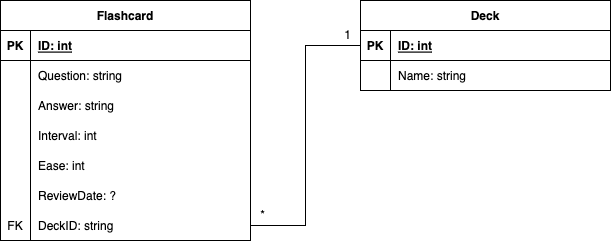
\includegraphics[width=0.9\textwidth]{NerddeckModel.png}
    \caption{Entity-Relationship Model of Flashcard and Deck}
    \label{fig:er-model}
\end{figure}

    \section{Functionalities}\label{sec:functionalities}
    \section{Target Users}\label{sec:target-users}
Users of this application could be every human for example students or teachers who want to remember something for a longer time. 


\chapter{Programming Languages Comparison}\label{chap:language-comparison}
In this chapter, we delve into the distinctive features of Go and Haskell, offering a brief overview of each language before embarking on comparative analysis.

    \section{Overview of Go}\label{sec:go-overview}
The usage of the programming language Go allows to build simple, secure and scalable systems. It is used very widely within big companys like Google, Paypal or Netflix. Besides of that it is open source. \cite{GoWebsite}
    \section{Overview of Haskell}\label{sec:haskell-overview}
Haskell is used for the comparison to Go because it is a pure functional programming language.
For the overview of Haskell the book \textit{Effective Haskell: Solving Real-World Problems with Strongly Typed Functional Programming} \cite{Skinner} will be used.
The first Haskell language report was published in 1990 by Paul Hudak and Philip Wadler. It is named after the mathematician Haskell Brooks Curry.\cite{Hudak2007}

    \section{Comparative Analysis}\label{sec:comparative-analysis}

\chapter{Implementation in Go}\label{chap:implementation-go}
    \section{Design Choices}\label{sec:design-go}
    \section{Code Structure}\label{sec:code-structure-go}
    \section{Key Features}\label{sec:key-features-go}
    \section{Challenges and Solutions}\label{sec:challenges-go}

\chapter{Implementation in Haskell}\label{chap:implementation-haskell}
    \section{Design Choices}\label{sec:design-haskell}
    \section{Code Structure}\label{sec:code-structure-haskell}
    \section{Key Features}\label{sec:key-features-haskell}
    \section{Challenges and Solutions}\label{sec:challenges-haskell}

\chapter{Functional Programming Paradigm in Practice}\label{chap:fp-paradigm}
    \section{Application of Functional Programming Concepts in Go}\label{sec:fp-go}
    \section{Application of Functional Programming Concepts in Haskell}\label{sec:fp-haskell}
    \section{Comparative Evaluation}\label{sec:fp-comparative}

\chapter{Modes of Operation}\label{chap:modes-operation}
    \section{Add New Cards}\label{sec:add-cards}
        \subsection{User Interface}\label{subsec:add-cards-ui}
        \subsection{Data Handling}\label{subsec:add-cards-data}
    \section{Learning Cards}\label{sec:learning-cards}
        \subsection{User Experience}\label{subsec:learning-cards-ux}
        \subsection{Algorithm for Learning}\label{subsec:learning-cards-algorithm}

\chapter{Consistency between Code and Documentation}\label{chap:consistency}
    \section{Code-Documentation Mapping}\label{sec:code-doc-mapping}
    \section{Ensuring Synchronization}\label{sec:synchronization}

\chapter{Conclusion}\label{chap:conclusion}
    \section{Summary of Findings}\label{sec:findings-summary}
    \section{Lessons Learned}\label{sec:lessons-learned}
    \section{Recommandations}
The book xy is recommended. The programming language xy is worth looking at.




%%% Local Variables: 
%%% mode: latex
%%% TeX-master: "thesis.tex"
%%% End: 
